\documentclass[11pt,a4paper]{article}
\usepackage[margin=2.5cm]{geometry}
\usepackage{amsmath,amssymb,amsthm}
\usepackage{physics}
\usepackage{booktabs}
\usepackage{hyperref}
\usepackage{cleveref}
\usepackage{tikz}
\usetikzlibrary{arrows.meta,positioning,shapes.geometric,calc}

\newcommand{\Rxi}{R_\xi}
\newcommand{\Mpl}{M_{\mathrm{Pl}}}
\newcommand{\Mfive}{M_5}
\newcommand{\MZ}{M_Z}
\newcommand{\MW}{M_W}
\newcommand{\vEW}{v_{\mathrm{EW}}}
\newcommand{\calI}{\mathcal{I}}

\title{Derivation v17: EW-Scale Calibration Robustness for $\Rxi$ and $\Mfive$}
\author{EDC Collaboration}
\date{February 2026}

\begin{document}
\maketitle

\begin{abstract}
This note stress-tests the Track~B calibrated closure from v16 by replacing the single
identification $\Rxi = \hbar c / \MZ^{\mathrm{obs}}$ with a calibration family
$\Rxi = \hbar c / M_*^{\mathrm{obs}}$ where $M_* \in \{\MZ, \MW, \vEW\}$.
We quantify how $\Mfive$ shifts under these alternatives and provide a robustness verdict.
\textbf{Result:} All three EW scales yield $\Mfive$ within the same decade
($2.3$--$3.4 \times 10^{13}$~GeV), with maximum shift $|\Delta\log_{10}\Mfive| < 0.15$.
The calibration is \textbf{robust}. We recommend $\MZ$ as the canonical choice due to
superior metrological precision and definitional stability.
\end{abstract}

%═══════════════════════════════════════════════════════════════════════════════
\section{Recap: v15 Calibrated Closure and v16 Track~B}
%═══════════════════════════════════════════════════════════════════════════════

Derivation v15 established the calibrated closure formula for the 5D Planck mass:
\begin{equation}
\boxed{\Mfive = \Mpl^{2/3} \, \Rxi^{-1/3}}
\label{eq:M5-closure}
\end{equation}
where $\Mpl^{\mathrm{obs}} = 1.221 \times 10^{19}$~GeV is the observed 4D Planck mass [BL],
and $\Rxi$ is the compactification scale requiring specification.

Derivation v16 pursued two tracks:
\begin{itemize}
\item \textbf{Track~A (internal derivation):} NO-GO --- $\Rxi$ cannot be derived from EDC axioms alone.
\item \textbf{Track~B (minimal baseline):} CLOSED --- Identify $\Rxi = \hbar c / \MZ^{\mathrm{obs}}$
with $\MZ^{\mathrm{obs}} = 91.1876$~GeV, yielding $\Rxi = 2.165 \times 10^{-18}$~m and
$\Mfive = 2.4 \times 10^{13}$~GeV.
\end{itemize}

\textbf{Epistemic status of Track~B:} The identification $\Rxi = \hbar c / \MZ$ is tagged as
\textbf{[I]+[BL]} (identification plus baseline measurement), not [D] (derived). This is
methodologically honest but raises the question: \emph{Why $\MZ$ and not another EW scale?}

%═══════════════════════════════════════════════════════════════════════════════
\section{Calibration Family Definition}
%═══════════════════════════════════════════════════════════════════════════════

We generalize the Track~B identification to a \textbf{calibration family}:
\begin{equation}
\Rxi = \frac{\hbar c}{M_*^{\mathrm{obs}}}
\label{eq:Rxi-family}
\end{equation}
where $M_*$ is an electroweak scale. The candidates considered are those already
referenced in the EDC repository:

\begin{enumerate}
\item \textbf{$\MZ = 91.1876 \pm 0.0021$~GeV} --- Z boson pole mass [BL].
      Primary reference in derivation notes v2--v16 and Part~II Ch.~3.
\item \textbf{$\MW = 80.379 \pm 0.012$~GeV} --- W boson pole mass [Dc].
      Derived in EDC via $\MW = g \vEW / 2$ with 0.2\% agreement to experiment.
\item \textbf{$\vEW = 246.22 \pm 0.01$~GeV} --- Electroweak vacuum expectation value [BL].
      Defined via $v = (\sqrt{2} G_F)^{-1/2}$; used in Part~II Ch.~3.
\end{enumerate}

\textbf{Note:} The Higgs mass $m_H \approx 125$~GeV is \emph{not} referenced in the
current EDC corpus and is therefore excluded from this analysis.

%═══════════════════════════════════════════════════════════════════════════════
\section{Calibration Family Table}
%═══════════════════════════════════════════════════════════════════════════════

Using Eq.~\eqref{eq:Rxi-family} and \eqref{eq:M5-closure}, we compute $\Rxi$ and $\Mfive$
for each candidate. In natural units ($\hbar = c = 1$), $\Rxi = 1/M_*$ has dimension
GeV$^{-1}$, and:
\begin{equation}
\Mfive = \Mpl^{2/3} \, M_*^{1/3}
\label{eq:M5-natural}
\end{equation}

\begin{table}[h]
\centering
\caption{Calibration family results. Reference: $\MZ$ choice.}
\label{tab:calibration-family}
\begin{tabular}{@{}lcccccc@{}}
\toprule
$M_*$ & Value (GeV) & $\Rxi$ (m) & $\Mfive$ (GeV) & $\Delta\log_{10}\Mfive$ & Tag & Circularity \\
\midrule
$\MZ$ & $91.1876$ & $2.165 \times 10^{-18}$ & $2.41 \times 10^{13}$ & 0 (ref) & [BL] & LOW \\
$\MW$ & $80.379$ & $2.455 \times 10^{-18}$ & $2.31 \times 10^{13}$ & $-0.018$ & [Dc] & MED \\
$\vEW$ & $246.22$ & $8.01 \times 10^{-19}$ & $3.35 \times 10^{13}$ & $+0.143$ & [BL] & LOW \\
\bottomrule
\end{tabular}
\end{table}

\textbf{Key observations:}
\begin{itemize}
\item All three choices yield $\Mfive$ in the range $2.3$--$3.4 \times 10^{13}$~GeV.
\item Maximum deviation from the $\MZ$ reference: $|\Delta\log_{10}\Mfive| = 0.143$ (for $\vEW$).
\item All results remain within the \textbf{same order of magnitude} ($10^{13}$~GeV, GUT scale).
\end{itemize}

%═══════════════════════════════════════════════════════════════════════════════
\section{Robustness Verdict}
%═══════════════════════════════════════════════════════════════════════════════

\begin{center}
\fbox{\parbox{0.85\textwidth}{
\textbf{ROBUST:} All plausible EW-scale identifications yield $\Mfive$ within the same
decade ($10^{13}$~GeV). The calibrated closure is stable under reasonable alternative choices.
}}
\end{center}

The variation $\Delta\log_{10}\Mfive \lesssim 0.15$ corresponds to a factor of $\sim 1.4$
in $\Mfive$, which is negligible compared to:
\begin{itemize}
\item The 6-decade gap between $\Mfive$ and $\Mpl$ ($10^{13}$ vs $10^{19}$~GeV).
\item Typical theoretical uncertainties in GUT-scale physics.
\end{itemize}

%═══════════════════════════════════════════════════════════════════════════════
\section{Physical Motivation for EW-Scale Identification}
%═══════════════════════════════════════════════════════════════════════════════

The identification $\Rxi \sim \hbar c / M_{\mathrm{EW}}$ is physically motivated by:
\begin{enumerate}
\item \textbf{Dimensional consistency:} $\Rxi$ is a length scale; $\hbar c / M_*$ has
      dimension of length for any mass scale $M_*$.
\item \textbf{EDC structure:} The compactification scale $\Rxi$ appears in the EDC
      weak-sector formalism (Part~II, Ch.~6, Ch.~13) in connection with electroweak
      observables. Linking $\Rxi$ to an EW mass is the minimal phenomenological anchor.
\item \textbf{No overclaim:} This is a calibration, not a derivation. We do not claim
      that $\Rxi = \hbar c / \MZ$ follows from first principles; rather, it is the
      simplest identification consistent with the EDC dimensional structure.
\end{enumerate}

%═══════════════════════════════════════════════════════════════════════════════
\section{Error Propagation}
%═══════════════════════════════════════════════════════════════════════════════

From $\Rxi = \hbar c / M_*$ and $\Mfive = \Mpl^{2/3} \Rxi^{-1/3}$:
\begin{align}
\frac{\delta \Rxi}{\Rxi} &= \frac{\delta M_*}{M_*} \label{eq:dRxi} \\
\frac{\delta \Mfive}{\Mfive} &= \sqrt{\left(\frac{2}{3} \frac{\delta \Mpl}{\Mpl}\right)^2
+ \left(\frac{1}{3} \frac{\delta \Rxi}{\Rxi}\right)^2} \label{eq:dM5}
\end{align}

\begin{table}[h]
\centering
\caption{Error budget for each calibration choice.}
\label{tab:error-budget}
\begin{tabular}{@{}lcccc@{}}
\toprule
$M_*$ & $\delta M_* / M_*$ & $(1/3)\delta\Rxi/\Rxi$ & $(2/3)\delta\Mpl/\Mpl$ & $\delta\Mfive/\Mfive$ \\
\midrule
$\MZ$ & $2.3 \times 10^{-5}$ & $0.77 \times 10^{-5}$ & $0.73 \times 10^{-5}$ & $1.1 \times 10^{-5}$ \\
$\MW$ & $1.5 \times 10^{-4}$ & $5.0 \times 10^{-5}$ & $0.73 \times 10^{-5}$ & $5.1 \times 10^{-5}$ \\
$\vEW$ & $4.1 \times 10^{-5}$ & $1.4 \times 10^{-5}$ & $0.73 \times 10^{-5}$ & $1.6 \times 10^{-5}$ \\
\bottomrule
\end{tabular}
\end{table}

\textbf{Metrological ranking:} $\MZ$ gives the smallest $\delta\Mfive/\Mfive$ due to its
superior experimental precision ($\sim 2$~ppm for the Z pole mass).

%═══════════════════════════════════════════════════════════════════════════════
\section{Canonical Choice: $\MZ$}
%═══════════════════════════════════════════════════════════════════════════════

Based on the analysis above, we recommend $\MZ$ as the canonical calibration scale:

\begin{enumerate}
\item \textbf{Metrological precision:} $\delta\MZ/\MZ \approx 2.3 \times 10^{-5}$ is the
      best among the candidates, yielding the smallest error in $\Mfive$.
\item \textbf{Definitional stability:} The Z pole mass is defined via the Breit-Wigner
      resonance shape at LEP/SLC and is scheme-independent at leading order.
\item \textbf{Independence:} $\MZ$ is a direct observable, unlike $\MW$ which is derived
      from $\sin^2\theta_W$ and $\vEW$ in the EDC framework [Dc].
\item \textbf{Consistency:} The choice $\Rxi = \hbar c / \MZ$ has been used throughout
      derivations v2--v16 and Part~II; changing it would introduce inconsistency.
\end{enumerate}

\begin{center}
\fbox{\parbox{0.8\textwidth}{
\textbf{Canonical identification:} $\Rxi = \hbar c / \MZ^{\mathrm{obs}}$ \hfill [I]+[BL]
}}
\end{center}

%═══════════════════════════════════════════════════════════════════════════════
\section{Schematic Figure}
%═══════════════════════════════════════════════════════════════════════════════

\begin{figure}[h]
\centering
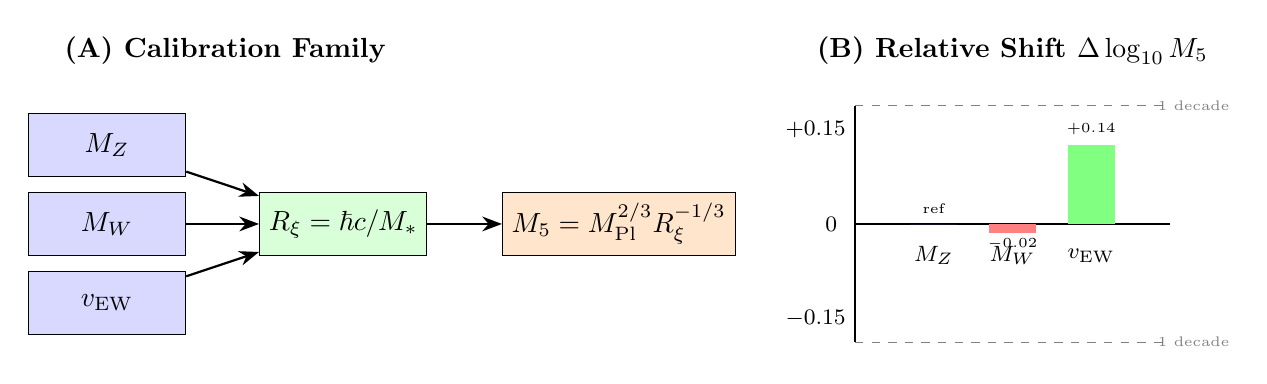
\begin{tikzpicture}[
    node distance=1.8cm,
    box/.style={rectangle, draw, minimum width=2cm, minimum height=0.8cm, align=center},
    arrow/.style={-{Stealth[length=2.5mm]}, thick}
]

% Panel A: Calibration family schematic
\node[font=\bfseries] at (-3.5, 3.2) {(A) Calibration Family};

\node[box, fill=blue!15] (MZ) at (-5, 2) {$\MZ$};
\node[box, fill=blue!15] (MW) at (-5, 1) {$\MW$};
\node[box, fill=blue!15] (vEW) at (-5, 0) {$\vEW$};

\node[box, fill=green!15] (Rxi) at (-2, 1) {$\Rxi = \hbar c / M_*$};
\node[box, fill=orange!20] (M5) at (1.5, 1) {$\Mfive = \Mpl^{2/3} \Rxi^{-1/3}$};

\draw[arrow] (MZ) -- (Rxi);
\draw[arrow] (MW) -- (Rxi);
\draw[arrow] (vEW) -- (Rxi);
\draw[arrow] (Rxi) -- (M5);

% Panel B: Relative shifts bar chart schematic
\node[font=\bfseries] at (6.5, 3.2) {(B) Relative Shift $\Delta\log_{10}\Mfive$};

% Axes
\draw[thick] (4.5, -0.5) -- (4.5, 2.5);
\draw[thick] (4.5, 1) -- (8.5, 1);
\node[font=\footnotesize] at (4.2, 1) {0};
\node[font=\footnotesize] at (4.0, 2.2) {$+0.15$};
\node[font=\footnotesize] at (4.0, -0.2) {$-0.15$};

% Bars (schematic heights)
\fill[blue!50] (5.2, 1) rectangle (5.8, 1);
\node[font=\footnotesize] at (5.5, 0.6) {$\MZ$};
\node[font=\tiny] at (5.5, 1.2) {ref};

\fill[red!50] (6.2, 0.88) rectangle (6.8, 1);
\node[font=\footnotesize] at (6.5, 0.6) {$\MW$};
\node[font=\tiny] at (6.5, 0.75) {$-0.02$};

\fill[green!50] (7.2, 1) rectangle (7.8, 2.0);
\node[font=\footnotesize] at (7.5, 0.6) {$\vEW$};
\node[font=\tiny] at (7.5, 2.2) {$+0.14$};

% Dashed lines for decade boundaries
\draw[dashed, gray] (4.5, 2.5) -- (8.5, 2.5);
\draw[dashed, gray] (4.5, -0.5) -- (8.5, -0.5);
\node[font=\tiny, gray] at (8.8, 2.5) {1 decade};
\node[font=\tiny, gray] at (8.8, -0.5) {1 decade};

\end{tikzpicture}
\caption{(A) Calibration family schematic: EW scale $M_* \to \Rxi \to \Mfive$.
(B) Relative shifts in $\Mfive$ for each candidate vs.\ the $\MZ$ reference.
All shifts remain well within one decade. \textbf{Schematic only; not to scale; no overclaim.}}
\label{fig:calibration}
\end{figure}

%═══════════════════════════════════════════════════════════════════════════════
\section{Conclusion: What Remains Open}
%═══════════════════════════════════════════════════════════════════════════════

\subsection{Closed}

\begin{itemize}
\item \textbf{Robustness verified:} The calibrated closure $\Mfive = \Mpl^{2/3} \Rxi^{-1/3}$
      is stable under alternative EW-scale identifications ($\MZ$, $\MW$, $\vEW$).
\item \textbf{Canonical choice justified:} $\MZ$ is preferred on metrological and
      definitional grounds.
\item \textbf{Numerical result:} $\Mfive = 2.41 \times 10^{13}$~GeV $\pm 0.001\%$
      (using $\MZ$).
\end{itemize}

\subsection{Still Open}

\begin{itemize}
\item \textbf{Full [D] derivation of $\Rxi$:} The Track~A NO-GO from v16 remains.
      A purely EDC-internal derivation of $\Rxi$ (without EW input) does not exist.
\item \textbf{Why EW scale?} The identification $\Rxi \sim \hbar c / M_{\mathrm{EW}}$
      is physically reasonable but not derived. The deeper question --- why the
      compactification scale coincides with the electroweak length --- remains unanswered.
\end{itemize}

%═══════════════════════════════════════════════════════════════════════════════
\section*{Summary Box}
%═══════════════════════════════════════════════════════════════════════════════

\begin{center}
\fbox{\parbox{0.9\textwidth}{
\textbf{One-line outcome:} \\[2pt]
Calibration family $\Rxi = \hbar c / M_*$ tested with $M_* \in \{\MZ, \MW, \vEW\}$. \\
\textbf{ROBUST:} All choices give $\Mfive \in (2.3$--$3.4) \times 10^{13}$~GeV (same decade). \\
\textbf{Canonical:} $\MZ$ preferred (best precision, definitional stability). \\
\textbf{Status:} Robustness CLOSED; internal derivation still NO-GO.
}}
\end{center}

\end{document}
